\documentclass{article}
\usepackage[utf8]{inputenc}
\usepackage[T1]{fontenc}
\usepackage{helvet}
\renewcommand{\thesubsubsection}{\thesubsection.\alph{subsubsection}}




\title{Mathebericht - Markov Ketten}
\author{Luis und Bas}
\date{2019}

\usepackage{natbib}
\usepackage{graphicx}
\usepackage{amsmath}
\usepackage{listings}
\usepackage{graphicx}
\usepackage{sectsty}
\usepackage{comment}
\usepackage{lmodern}
\usepackage{textcomp}
\usepackage{chemformula}
\usepackage{booktabs}
\usepackage{float}
\usepackage{chemformula}

\begin{document}

\maketitle


\section{Markov Ketten: Wahrscheinlichkeit beim Tennis}
\subsection{Tennis Match 1}
\subsubsection{} Als Zusatzblatt
\subsubsection{} 
\[
M=
  \begin{pmatrix}
    0 & 0.4 & 0.6 & 0 & 0 \\
    0.6 & 0 & 0 & 0 & 0 \\
    0.4 & 0 & 0 & 0 & 0 \\
    0 & 0.6 & 0 & 1 & 0 \\
    0 & 0 & 0.4 & 0 & 1
    
  \end{pmatrix}
\]
\subsubsection{}
\[
M=
  \begin{pmatrix}
    -1 & 0.4 & 0.6 & 0 & 0 \\
    0.6 & -1 & 0 & 0 & 0 \\
    0.4 & 0 & -1 & 0 & 0 \\
    0 & 0.6 & 0 & 0 & 0 \\
    0 & 0 & 0.4 & 0 & 0
    
  \end{pmatrix}
\]

\vspace{5mm}
Gleichungen: \\
Zeile 1: a = 0.4b + 0.6c \\
Zeile 2: b = 0.6a \\
Zeile 3: c = 0.4a \\
Zeile 4: b = 0 \\
Zeile 5: c = 0 \\

\vspace{5mm}
a, b, c = 0
Gleichungsystem doppelt unterbestimmt -> Fläche

\[
w1=
  \begin{pmatrix}
    0 \\
    0 \\
    0 \\
    1 \\
    0 
    
  \end{pmatrix}
\]
\[
w2=
  \begin{pmatrix}
    0 \\
    0 \\
    0 \\
    0 \\
    1 
    
  \end{pmatrix}
\]

\subsubsection{}
\[
v=
  \begin{pmatrix}
    1 \\
    0 \\
    0 \\
    0 \\
    0 
    
  \end{pmatrix}
\]

\[
P^3 * v=
  \begin{pmatrix}
    0.00000 \\
    0.28800 \\
    0.19200 \\
    0.36000 \\
    0.16000 \\
    
  \end{pmatrix}
\]
Erklärung: \\
Dies sind die Wahrscheinlichkeiten für die verschiedenen Zustände nach 3 Schritten.

\subsubsection{}
\[
u=
  \begin{pmatrix}
    0 \\
    1 \\
    0 \\
    0 \\
    0 
    
  \end{pmatrix}
\]

\[
P^3 * u=
  \begin{pmatrix}
    0.19200 \\
    0.00000 \\
    0.00000 \\
    0.74400 \\
    0.06400 \\
    
  \end{pmatrix}
\]
\[
P^{30} * u=
  \begin{pmatrix}
    0.00000 \\
    0.00001 \\
    0.00001 \\
    0.87691 \\
    0.12307 \\
    
  \end{pmatrix}
\]
\[
P^{100} * u=
  \begin{pmatrix}
    0.00000 \\
    0.00000 \\
    0.00000 \\
    0.87692 \\
    0.12308 \\
    
  \end{pmatrix}
\]
Erklärung: \\
Bei $P^3$ ist noch ein gewisser Teil der Spiele im Einstand, während bei $P^{30}$ und $P^{100}$ (fast) alle Spiele schon beendet und meistens zugunsten von Spieler 1 ausgegangen sind.

\subsubsection{}

Lösungsweg: \\
\vspace{5mm}
\footnotesize{
\begin{lstlisting}
Funktion "f": 
function y = f (x) 
  V = [ 
   0.00000   0.00000  -0.67479  -0.00000   0.42602; 
   0.00000   0.00000   0.58438  -0.73019   0.36894; 
   0.00000   0.00000   0.38959   0.48679   0.24596; 
   1.00000   0.00000  -0.20713   0.43811  -0.72064; 
   0.00000   1.00000  -0.09206  -0.19472  -0.32028; 
  ] 
  goal = [1; 0; 0; 0; 0] 
  y = zeros(5,1) 
  y(1) = x(1) * V(1,1) + x(2) * V(1,2) + x(3) * V(1,3) + x(4) * V(1,4) + x(5) * V(1,5) - 1 
  y(2) = x(1) * V(2,1) + x(2) * V(2,2) + x(3) * V(2,3) + x(4) * V(2,4) + x(5) * V(2,5) 
  y(3) = x(1) * V(3,1) + x(2) * V(3,2) + x(3) * V(3,3) + x(4) * V(3,4) + x(5) * V(3,5) 
  y(4) = x(1) * V(4,1) + x(2) * V(4,2) + x(3) * V(4,3) + x(4) * V(4,4) + x(5) * V(4,5) 
  y(5) = x(1) * V(5,1) + x(2) * V(5,2) + x(3) * V(5,3) + x(4) * V(5,4) + x(5) * V(5,5) 
endfunction
\end{lstlisting}
}
\begin{lstlisting}
Datei "tennis1": 
P = [0, 0.4, 0.6, 0, 0; 
    0.6, 0, 0, 0, 0; 
    0.4, 0, 0, 0, 0; 
    0, 0.6, 0, 1, 0; 
    0, 0, 0.4, 0, 1] 
[x, fval, info] = fsolve (@f, [1; 1; 1; 1; 1]) 
\end{lstlisting}
\vspace{5mm}
\normalsize
Output von "tennis1":
\[
x=
  \begin{pmatrix}
    0.6923066298 \\
    0.3076859606 \\
    -0.7409688692 \\
    0.0000025369 \\
    1.1736576142 \\
    
  \end{pmatrix}
\]

\subsubsection{}

$\lim\limits_{n \rightarrow \infty}{M^n} = M^n * v =$ \[
  \begin{pmatrix}
    z1 \\
    z2 \\
    z3 \\
    z4 \\
    z5 \\
  \end{pmatrix}
\]
\\
z4 gesucht! \\ \\
\vspace{5mm}
$\lim\limits_{n \rightarrow \infty}{M^n * v} = M^n * x_1 * w_1 + M^n * x_2 * w_2 ... + M^n * x_5 * w_5 \\
= \lambda_1 * x_1 * w_1 + \lambda_2 * x_2 * w_2 ... + \lambda_5* x_5 * w_5 \\$
\vspace{5mm} \\
Weil: $\lambda_1 = \lambda_2 = 0$ und  $\lambda_3 < 0$, $\lambda_4 < 0$, $\lambda_5 < 0$\\
\vspace{5mm} \\
$\lim\limits_{n \rightarrow \infty}{M^n * v} = x_1 * w_1  + x_2 * w_2 = endvektor$ \\
 \\
$endvektor_4 = 0.69231$


\subsubsection{}
$P^{10000} * v$ = \[
  \begin{pmatrix}
    0 \\
    0 \\
    0 \\
    0.69231 \\
    0.30769 \\
    
  \end{pmatrix}
\]

Chance $= 69.231 \%$


\subsection{Tennis Match 2}
\subsubsection{}
\begin{lstlisting}
function P = prob_win (p)
  P = [0, 1-p, p, 0, 0;
      p, 0, 0, 0, 0;
      1-p, 0, 0, 0, 0;
      0, p, 0, 1, 0;
      0, 0, 1-p, 0, 1]
endfunction
\end{lstlisting}

\subsubsection{}
\begin{lstlisting}
function [P, lincomb] = prob_win (p, v)
  P = [0, 1-p, p, 0, 0;
      p, 0, 0, 0, 0;
      1-p, 0, 0, 0, 0;
      0, p, 0, 1, 0;
      0, 0, 1-p, 0, 1];
  
  [w, LAMBDA] = eig(P);
  
  lincomb = w \ v;
endfunction
\end{lstlisting}

\subsubsection{}
\begin{lstlisting}
function [P, lincomb, win_chance] = prob_win (p, v)
  P = [0, 1-p, p, 0, 0;
      p, 0, 0, 0, 0;
      1-p, 0, 0, 0, 0;
      0, p, 0, 1, 0;
      0, 0, 1-p, 0, 1];
  
  [w, LAMBDA] = eig(P);
  
  lincomb = w \ v;
  
  win_chance = lincomb(1);
endfunction
\end{lstlisting}

\subsubsection{}
Kleines Umschreiben von "prob\_win.m": \\
\begin{lstlisting}
function [win_chance, lincomb, P] = prob_win (p, v)
  P = [0, 1-p, p, 0, 0;
      p, 0, 0, 0, 0;
      1-p, 0, 0, 0, 0;
      0, p, 0, 1, 0;
      0, 0, 1-p, 0, 1];
  
  [w, LAMBDA] = eig(P);
  
  lincomb = w \ v;
  
  win_chance = lincomb(1);
endfunction
\end{lstlisting}

tennis2.m: \\
\begin{lstlisting}
v = eye(5,1);
k = [];
o = [];
for i=1:100
	win_chance = prob_win((i-1)/100, v);
	k(i) = win_chance;
  o(i) = (i-1)/100;
endfor
plot(o, k)
\end{lstlisting}

\begin{figure}[h!]
\centering
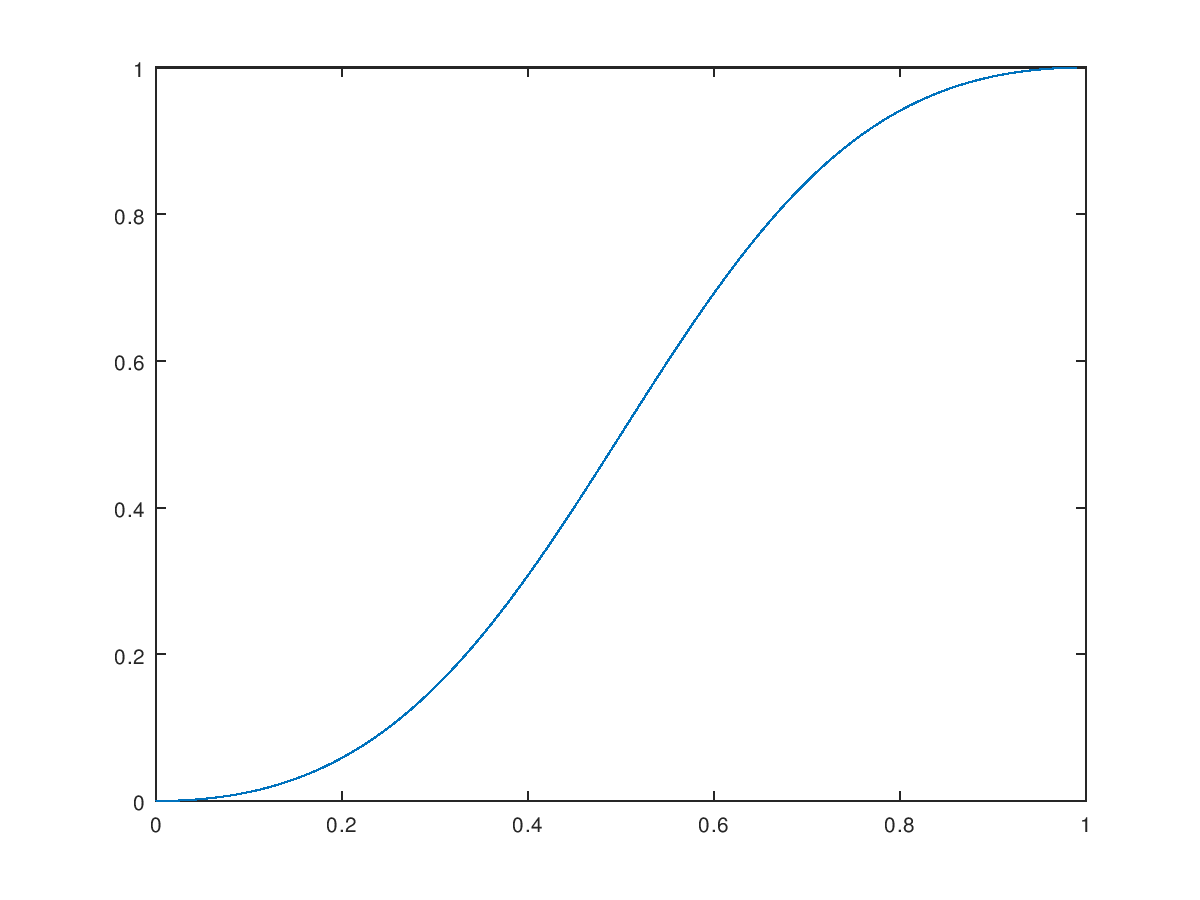
\includegraphics[scale=0.4]{graph.png}
\caption{Graph von tennis2.m}
\label{fig:universe}
\end{figure}

\subsubsection{}
tennis2\_alle.m: \\
\begin{lstlisting}
hold on;

v = eye(5,1);
k = [];
o = [];
for i=1:100
	win_chance = prob_win((i-1)/100, v);
	k(i) = win_chance;
  o(i) = (i-1)/100;
endfor
plot(o, k)

v = [0;1;0;0;0];
k = [];
o = [];
for i=1:100
	win_chance = prob_win((i-1)/100, v);
	k(i) = win_chance;
  o(i) = (i-1)/100;
endfor
plot(o, k)

v = [0;0;1;0;0];
k = [];
o = [];
for i=1:100
	win_chance = prob_win((i-1)/100, v);
	k(i) = win_chance;
  o(i) = (i-1)/100;
endfor
plot(o, k)

\end{lstlisting}

\begin{figure}[h!]
\centering
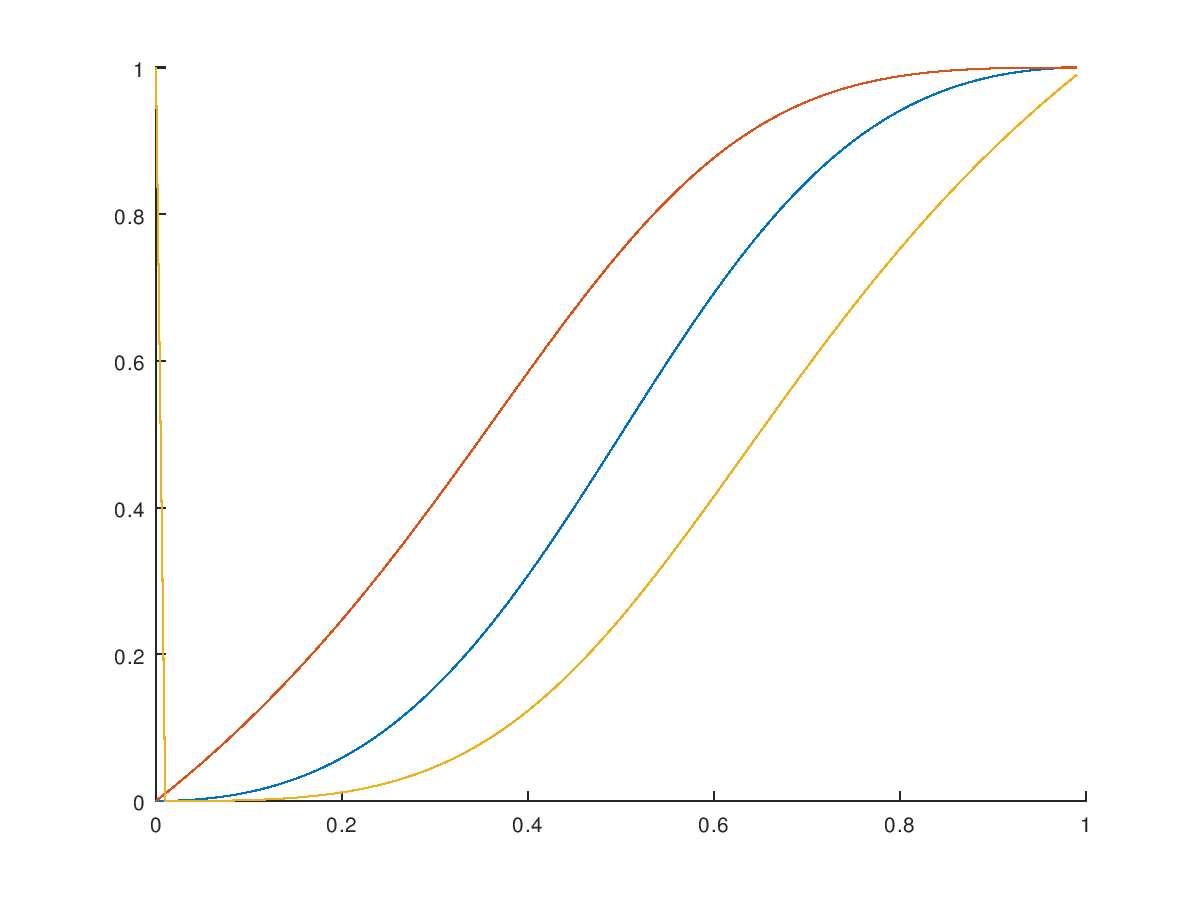
\includegraphics[scale=0.4]{graph2.png}
\caption{Graph von tennis2\_alle.m}
\label{fig:universe}
\end{figure}

\subsection{Tennis Match 3}

\subsubsection{}
Chance auf Einstand:

1 - (Chance auf Sieg + Chance auf Niederlage)

$= 1 - (p^2 + (1-p)^2)$

$= 1 - (p^2 + 1 - 2p + p^2)$

$= 1 - 2p^2 - 1 + 2p$

$= 2p - 2p^2$

\subsubsection{}
Chance auf Sieg nach drei weitere Einstände:

$($Chance auf Einstand$)^3 * ($Chance auf Sieg$)$

$= (2p - 2p^2)^3 * p^2$

\subsubsection{}
Berechnung der Siegeschance:

$$\lim_{n\to\infty} \sum_{k=0}^{n} p^2 * (2p-2p^2)^k$$

Geometrische Folge:

\[=\frac{p^2}{1-(2p-2p^2)}\]

\[=\frac{0.6^2}{1-(2*0.6-2*(0.6^2))}\]

\[=\frac{0.36}{1-(1.2-0.72)}\]

\[=0.6923076923\]

\subsubsection{}

\begin{lstlisting}
function winChance = hand_win (p)
  winChance = (p*p)/(2*(p**2) - 2*p + 1)
endfunction


p = 0:0.01:1;
w = [];

for i = 1:101
   w(i) = hand_win(p(i));
endfor

plot(0:0.01:1, w)
\end{lstlisting}

\begin{figure}[h!]
\centering
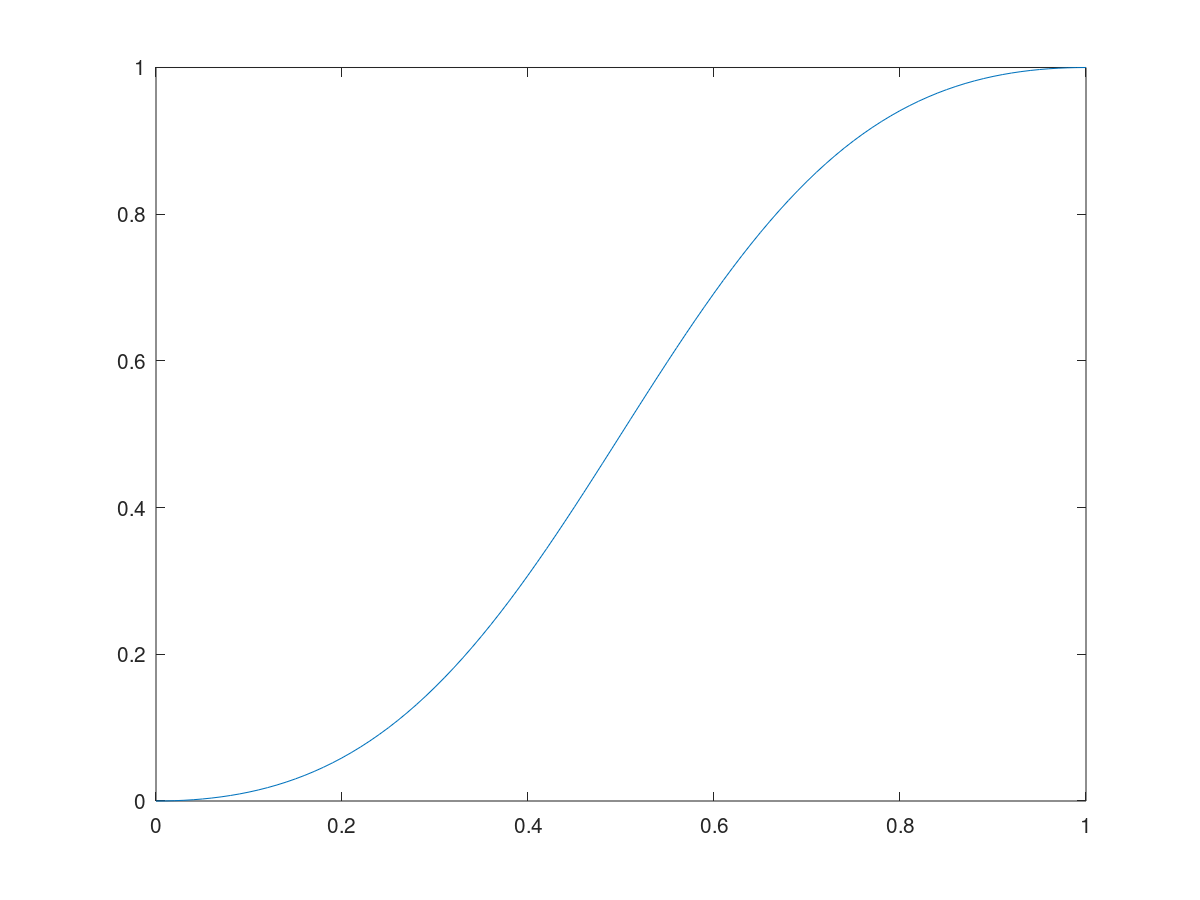
\includegraphics[scale=0.2]{winplot.png}
\caption{Winchance}
\label{fig:universe}
\end{figure}




\section{Populationsmodelle}
\subsubsection{}
Auf Zusatzblatt
\subsubsection{}
Bleibt konstant \\
Erklärung: Es kommen immer 6 dazu, danach durch 2 und durch 3 -> wieder bei 1
\subsubsection{}
eig(A1) = 2, -1, -1 -> wird immer grösser, dominanter (=absolut gesehen grösster) > 1 \\
eig(A2) = 0.75, 0.375, 0.375 -> wird immer kleiner, dominanter (=absolut gesehen grösster) < 1 \\
eig(A3) = 1, -0.5, -0.5 -> bleibt konstant, dominanter (=absolut gesehen grösster) = 1 \\
%eig(A4) = 1, -1 -> bleibt gleich \\
\subsubsection{}
plot\_pop\_sum.m:
\begin{lstlisting}
function endmatrix = plot_pop_sum (M)
  endmatrix = zeros(1,11);
  for i=0:10
    v = ones(size(M)(1),1) * 10;
    endmatrix(1,i+1) = sum(M^i * v);
  endfor
  endmatrix
  plot(0:10,endmatrix)
endfunction
\end{lstlisting}

\begin{figure}[H]
\centering
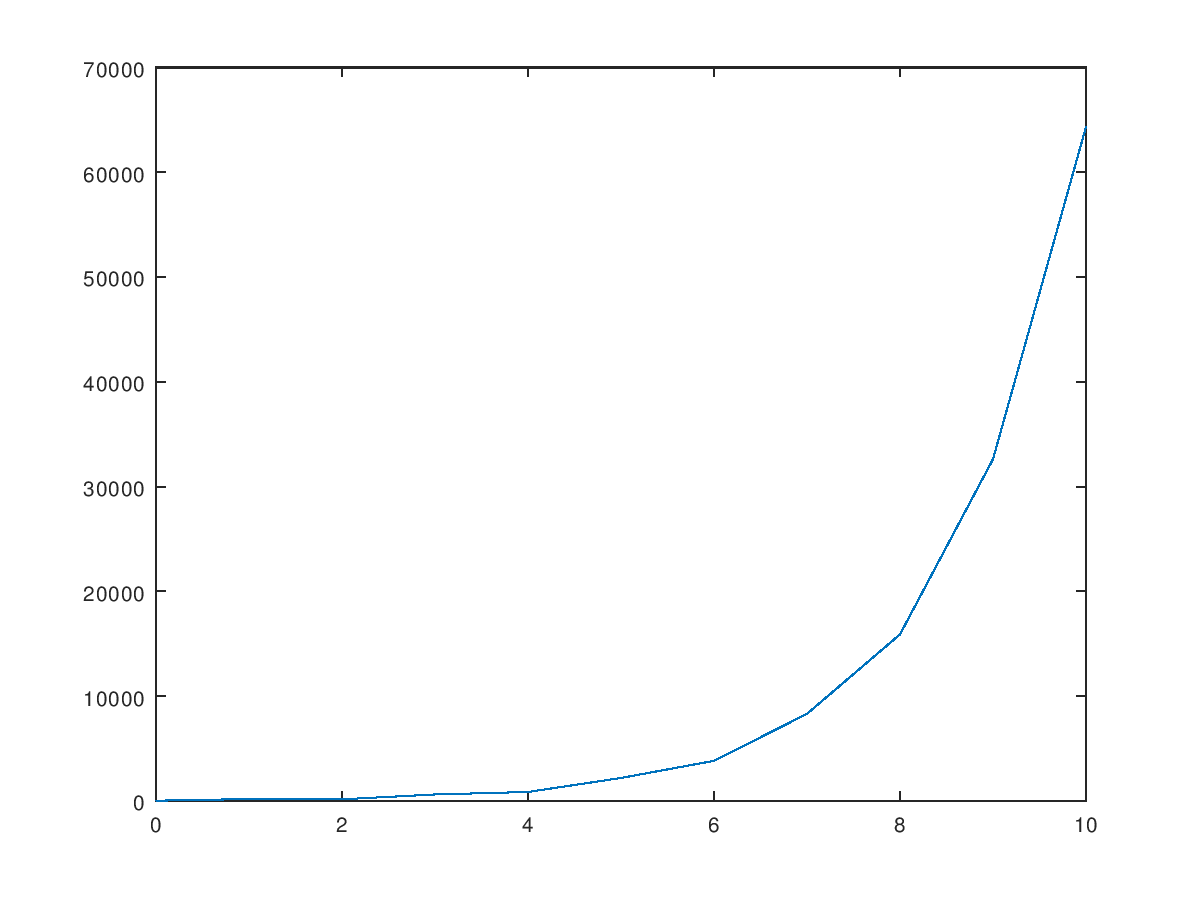
\includegraphics[scale=0.6]{plotA1.png}
\caption{plot\_pop\_sum(A1)}
\label{fig:universe}
\end{figure}

\begin{figure}[H]
\centering
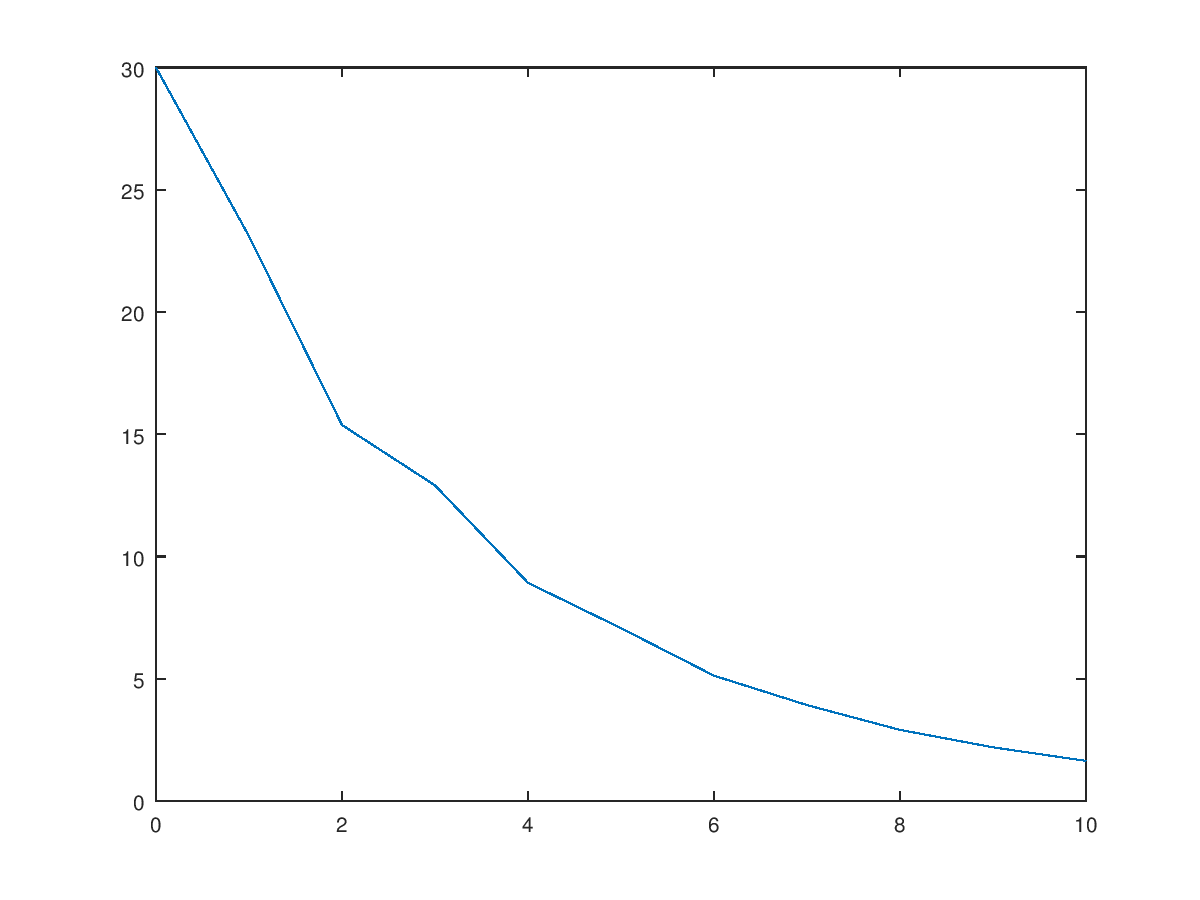
\includegraphics[scale=0.5]{plotA2.png}
\caption{plot\_pop\_sum(A2)}
\label{fig:universe}
\end{figure}

\begin{figure}[H]
\centering
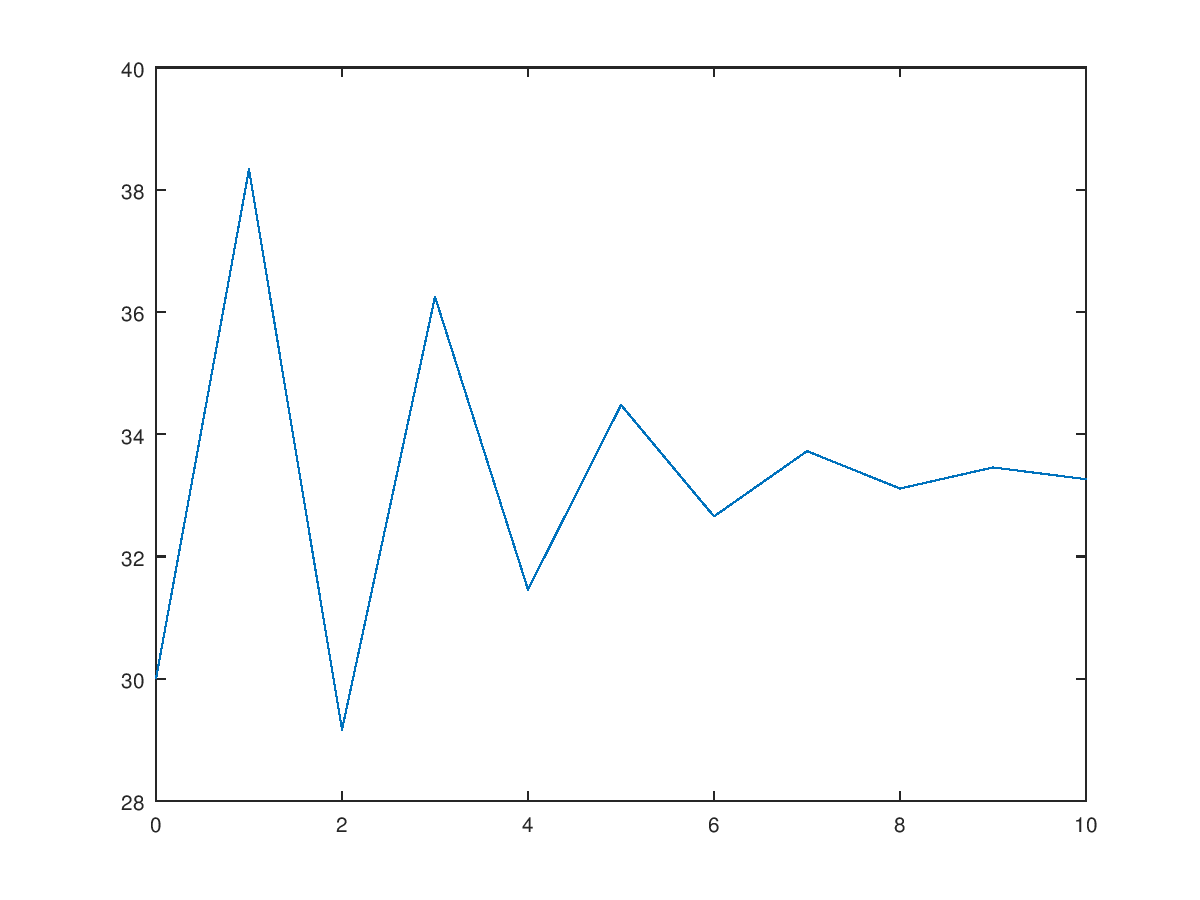
\includegraphics[scale=0.5]{plotA3.png}
\caption{plot\_pop\_sum(A3)}
\label{fig:universe}
\end{figure}

\begin{figure}[H]
\centering
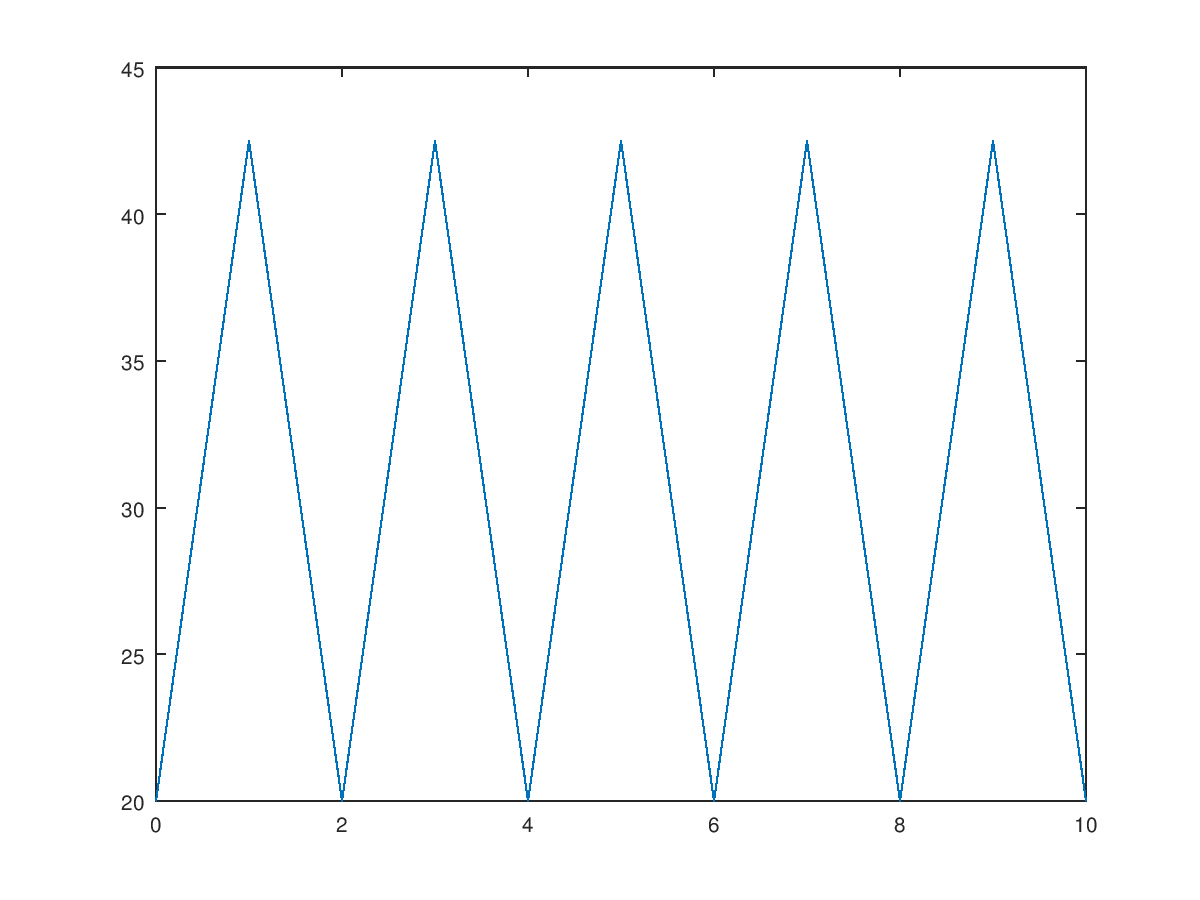
\includegraphics[scale=0.5]{plotA4.png}
\caption{plot\_pop\_sum(A4)}
\label{fig:universe}
\end{figure}

\begin{figure}[H]
\centering
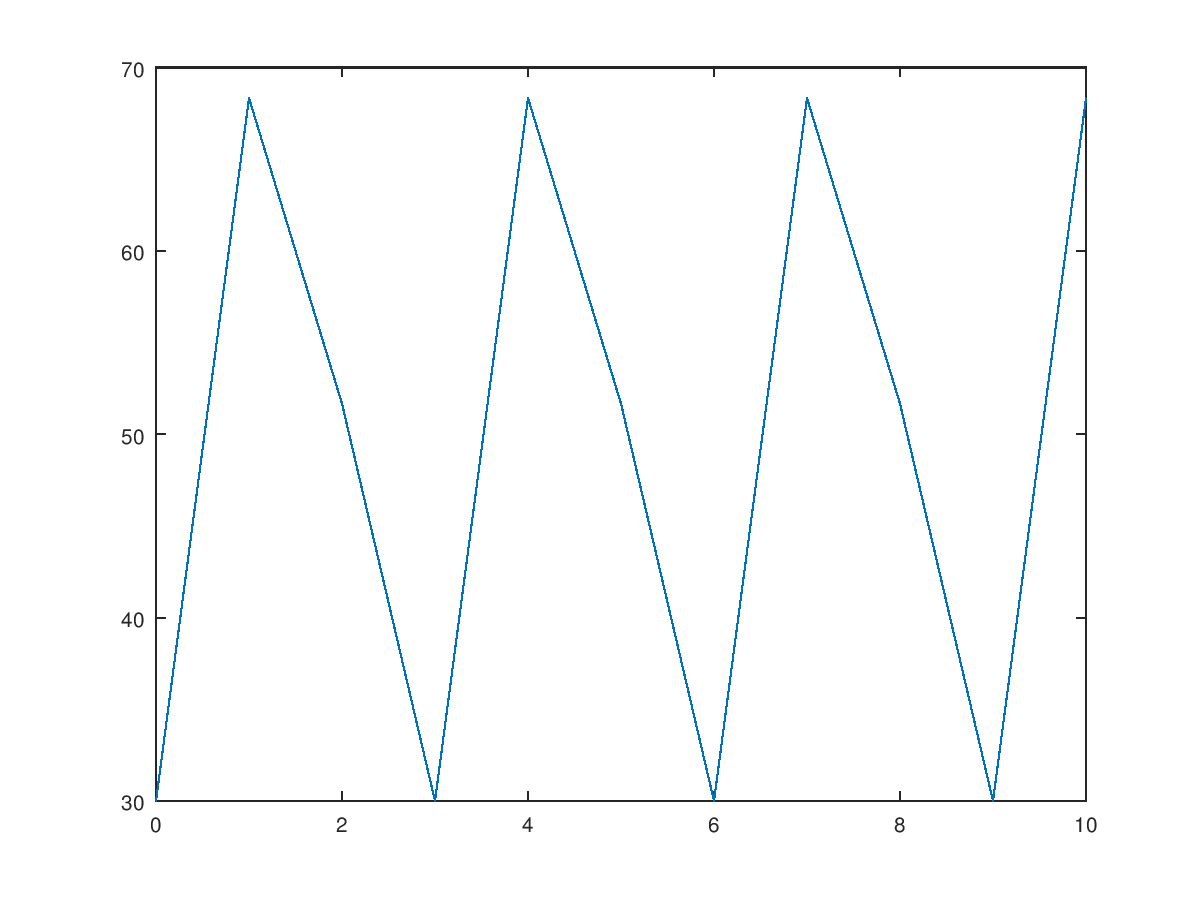
\includegraphics[scale=0.5]{plotA5.png}
\caption{plot\_pop\_sum(A5)}
\label{fig:universe}
\end{figure}

\subsubsection{}
plot\_pop\_rel.m:
\begin{lstlisting}
function endmatrix = plot_pop_rel (M)
  endmatrix = zeros(size(M)(1),11);
  for i=0:10
    v = ones(size(M)(1),1) * 10;
    res = M^i * v;
    endmatrix(:,i+1) = res / sum(res);
  endfor
  endmatrix
  plot(0:10,endmatrix(1,:), 0:10, endmatrix(2,:), 0:10, endmatrix(3,:))
endfunction
\end{lstlisting}

\begin{figure}[H]
\centering
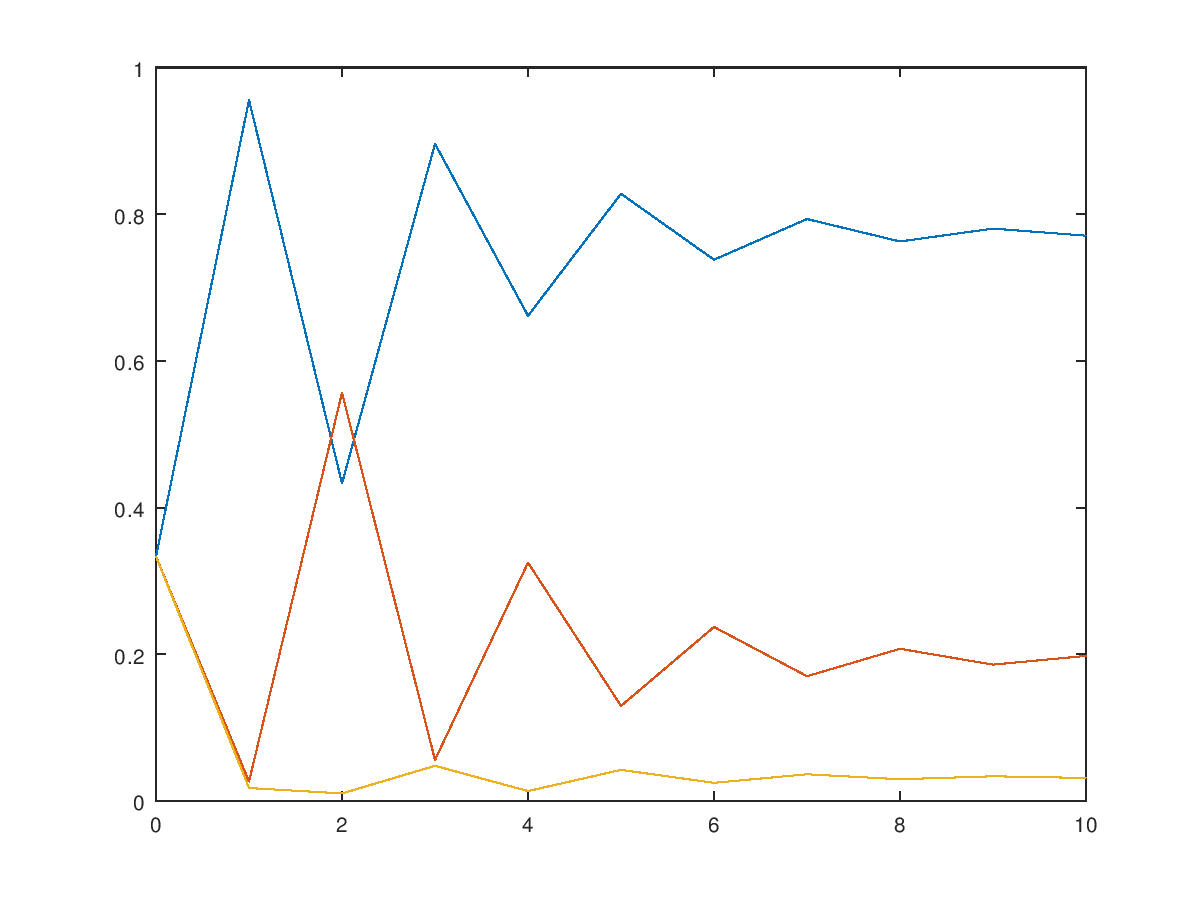
\includegraphics[scale=0.5]{plotrelA1.png}
\caption{plot\_pop\_rel(A1)}
\label{fig:universe}
\end{figure}

\begin{figure}[H]
\centering
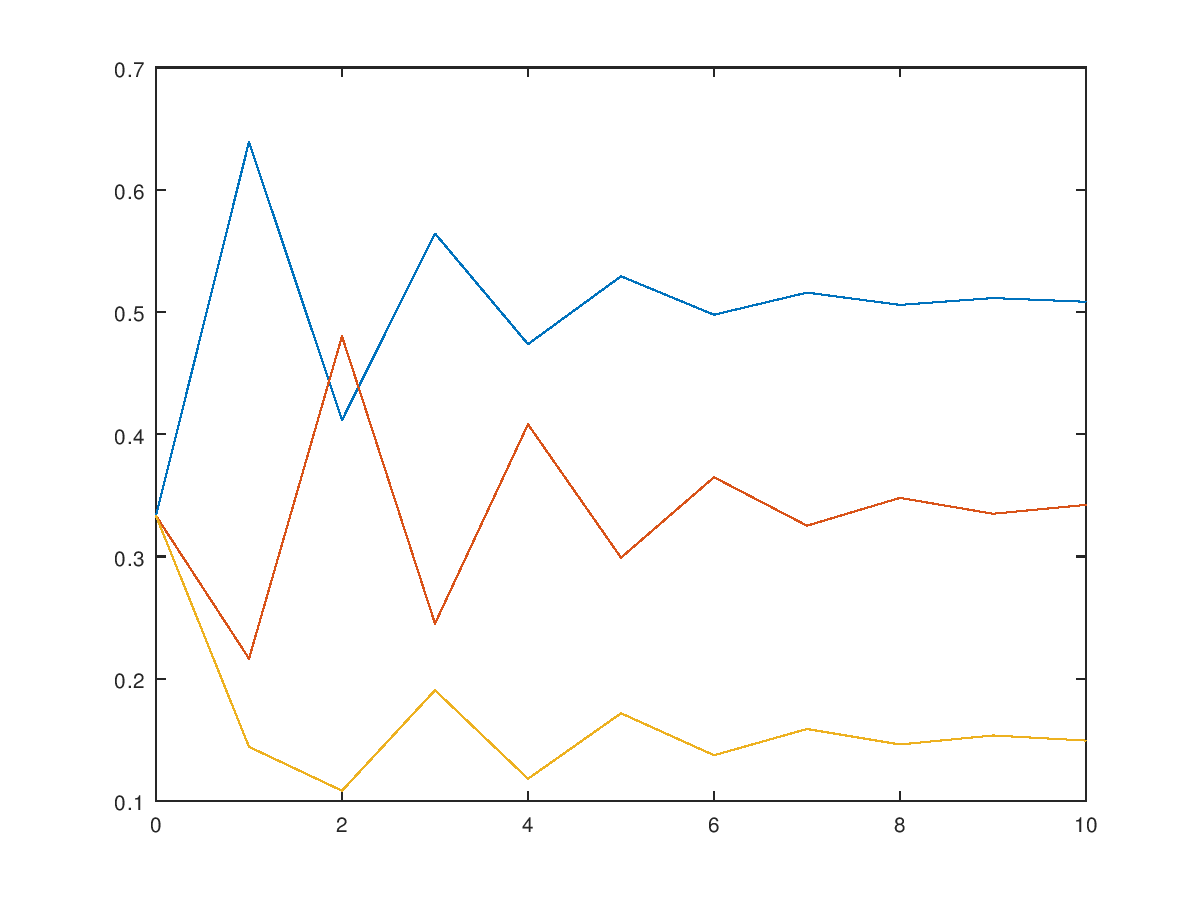
\includegraphics[scale=0.5]{plotrelA2.png}
\caption{plot\_pop\_rel(A2)}
\label{fig:universe}
\end{figure}

\begin{figure}[H]
\centering
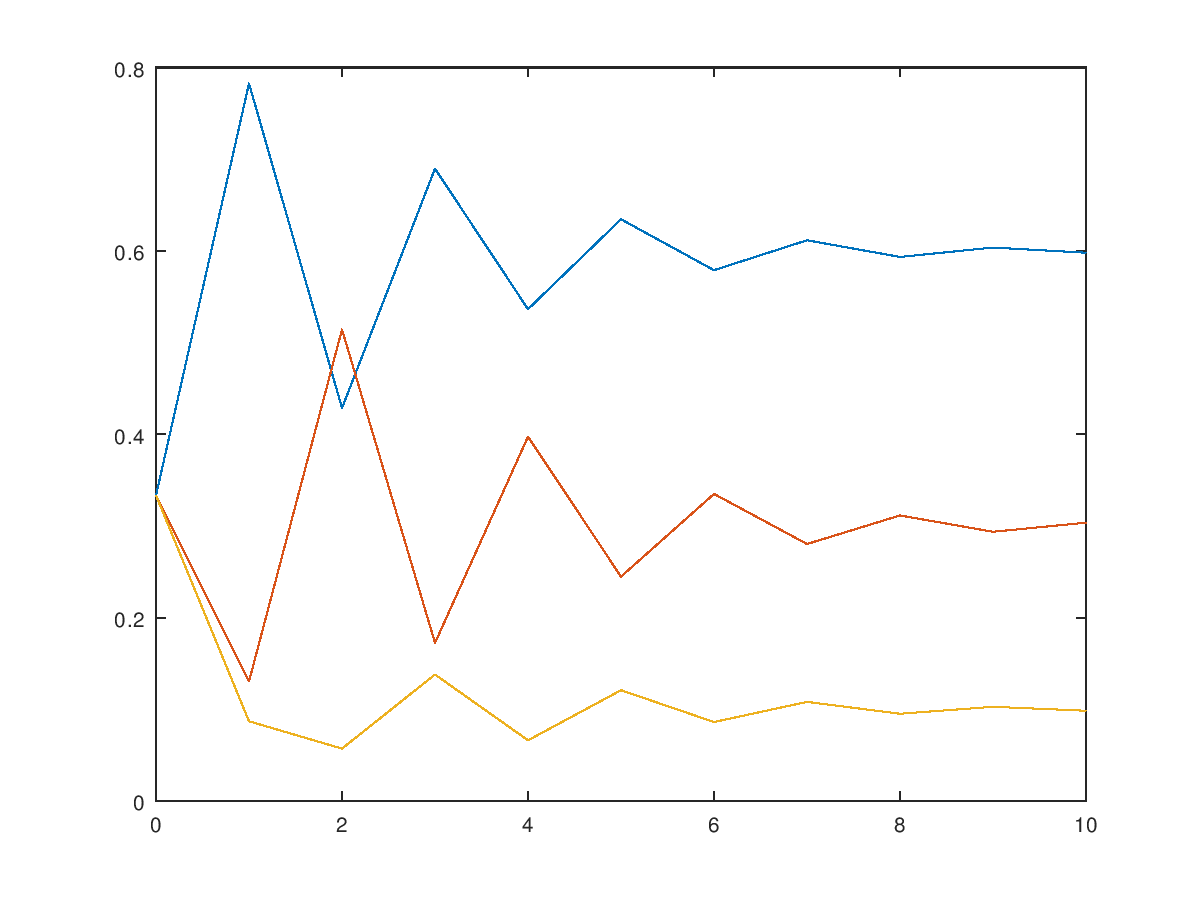
\includegraphics[scale=0.5]{plotrelA3.png}
\caption{plot\_pop\_rel(A3)}
\label{fig:universe}
\end{figure}

\subsubsection{}
Am Beispiel A1: \\
[V, LAM] = eig(A1)
\[
V =
  \begin{pmatrix}
    -0.96935 + 0.00000i && 0.88465 + 0.00000i && 0.88465 - 0.00000i \\ 
    -0.24234 + 0.00000i && -0.44233 - 0.00000i && -0.44233 + 0.00000i \\
    -0.04039 + 0.00000i &&  0.14744 + 0.00000i && 0.14744 - 0.00000i \\
  \end{pmatrix}
\]
\[
LAM =
  \begin{pmatrix}
    2.00000 + 0.00000i && 0 && 0 \\ 
    0 && -1.00000 + 0.00000i && 0 \\
    0 &&  0 &&  -1.00000 - 0.00000i \\
  \end{pmatrix}
\]

Der Eigenwert \textbf{2} ist der dominate Eigenwert und wird langfristig gesehen der einzig wichtige Eigenvektor sein. Dessen dazugehöriger Eigenvektor zeigt deshalb auch die Aufteilung der Population langfristig gesehen.

\subsubsection{}
Die Eigenwerte von A4 = [1, -1] und A5 = [-0.5 + 0.86603i, -0.5 + 0.86603i, 1] haben alle den gleichen Betrag (=1). Es gibt keinen dominaten Eigenwert und man muss alle berücksichtigen.

\subsubsection{}
Sage man habe die Matrix M und deren Eigenwerte $\lambda_1, \lambda_2 ... \lambda_n$ \\
Man berechne nun für jeden Eigenwert $\lambda_k$ den Betrag $|\lambda_k|$. Gibt es einen Eigenwert welcher grösser ist als alle anderen so ist nur dieser wichtig. Sind die Beträge mehrer Eigenwerte gleich gross, so sind alle dominant und müssen berücksichtigt werden.

\vspace{5mm}

$Wachstum = \left\{
\begin{array}{ll}
|\lambda_{dom}| > 1 & \, \textrm{Population wird immer grösser} \\
|\lambda_{dom}| < 1 & \, \textrm{Population wird immer kleiner} \\
|\lambda_{dom}| = 1 & \, \textrm{Population pendelt sich ein, bleibt gleich} \\
\end{array}
\right. $

\subsubsection{}

eig\_dom.m:
\begin{lstlisting}
function dom = eig_dom (M)
  LAM = eig(M);
  big = 0;
  dom = [];
  
  for i=1:(size(LAM)(1))
    cur = abs(LAM(i));
    if big > cur
      continue
    elseif big == cur
      dom(size(dom)(1)+1,1) = LAM(i);
    else
      dom = [LAM(i)];
      big = cur;
    endif
  endfor
endfunction
\end{lstlisting}

\subsection{Schutz für die Unechte Karettschildkröte 1}
\subsubsection{}
Die Perioden haben eine unterschiedliche Dauer, also gehen nicht alle Überlebende einer Gruppe in die nächste Gruppe.

\subsubsection{}
Der Wert bedeutet, dass nach einem Jahr 66.11\% aller grosser Jugenlichen immer noch grosse Jugendliche sind.

\subsubsection{}

pop\_karettschildkroete.m:


\begin{lstlisting}
L = [ 0       0         0         0         127       4         80;
      0.6747  0.7371    0         0         0         0         0;
      0       0.0486    0.6611    0         0         0         0;
      0       0         0.0147    0.6907    0         0         0;
      0       0         0         0.0518    0         0         0;
      0       0         0         0         0.8091    0         0;
      0       0         0         0         0         0.8091    0.8088;
      ];
v0 = [10000; 10000; 10000; 10000; 10000; 10000; 10000];

r = zeros(50,1);

for i = 1:50
  t = L^i * v0;
  r(:,i) = t;
endfor

hold on
for i = 1:7
  plot(1:50, r(i,:));
endfor
hold off
\end{lstlisting}

\begin{figure}[H]
\centering
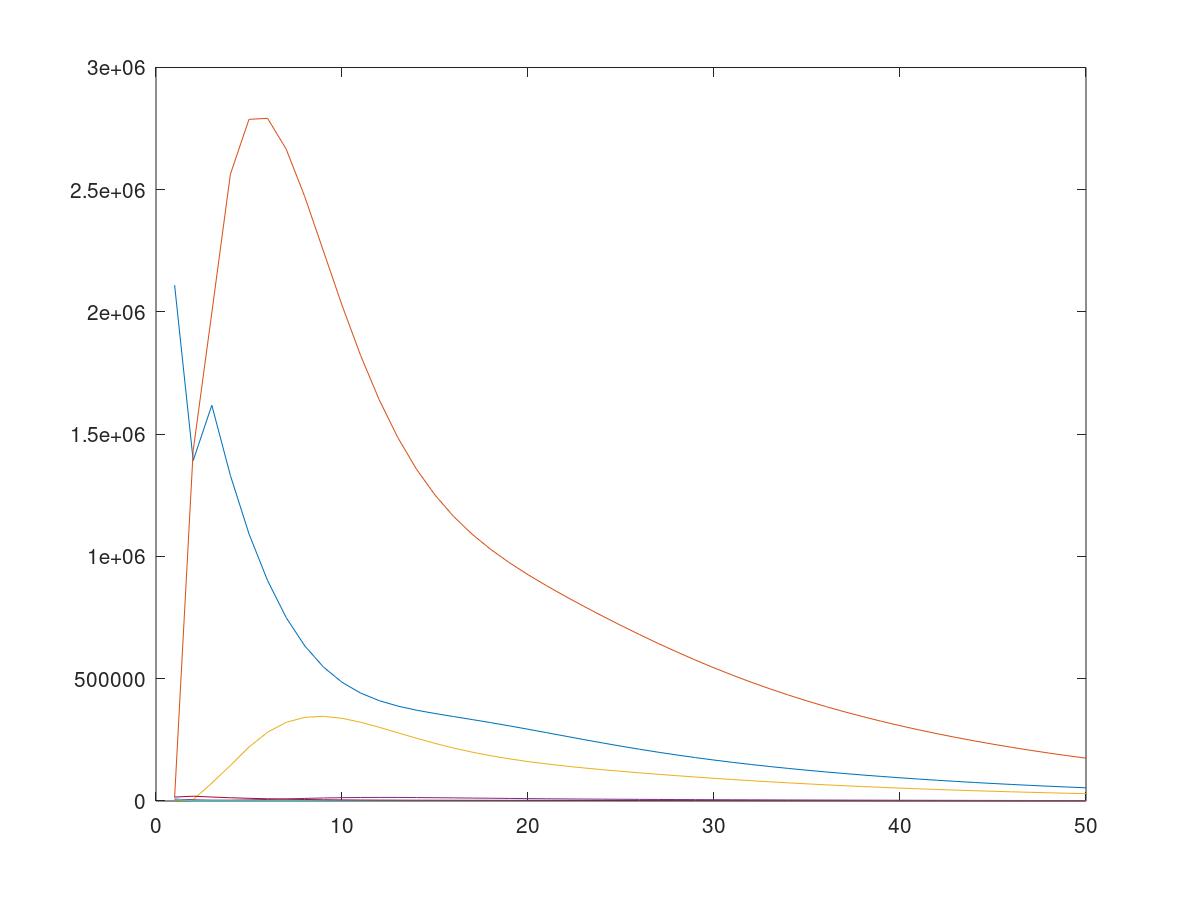
\includegraphics[scale=0.3]{plotK1c.png}
\label{fig:universe}
\caption{Population Karettschildkröte}
\end{figure}


\subsubsection{}
L = \begin{pmatrix}
    0 & 0 & 0 & 0 & 127 & 4 & 80 \\
    1 & 0.7371 & 0 & 0 & 0 & 0 & 0 \\
    0 & 0.0486 & 0.6611 & 0 & 0 & 0 & 0 \\
    0 & 0 & 0.0147 & 0.6907 & 0 & 0 & 0 \\
    0 & 0 & 0 & 0.0518 & 0 & 0 & 0 \\
    0 & 0 & 0 & 0 & 0.8091 & 0 & 0 \\
    0 & 0 & 0 & 0 & 0 & 0.8091 & 0.8088 \\
  \end{pmatrix}

\subsubsection{}


\begin{lstlisting}
L = [0,0,0,0,127,4,80;
1,0.7371,0,0,0,0,0;
0,0.0486,0.6611,0,0,0,0;
0,0,0.0147,0.6907,0,0,0;
0,0,0,0.0518,0,0,0;
0,0,0,0,0.8091,0,0;
0,0,0,0,0,0.8091,0.8088];

eig_dom(L)(1,1)

\end{lstlisting}
Output: 0.96497, das heisst
auch wenn Eier und Jungtiere geschützt werden, stirbt die Population aus.

\subsubsection{}
\begin{lstlisting}
function M = x_abhangig_schild (x)
  M = [0,0,0,0,127,4,80;
    0.6747,0.7371,0,0,0,0,0;
    0,0.0486,0.6611,0,0,0,0;
    0,0,0.0147,0.6907 * x,0,0,0;
    0,0,0,0.0518 * x,0,0,0;
    0,0,0,0,0.8091 * x,0,0;
    0,0,0,0,0,0.8091 * x,0.8088 * x];
endfunction


fin = [];

for i=1:100
  cur = i/10;
  M = x_abhangig_schild(cur);
  fin(i) = eig_dom(M)(1,1);
endfor

plot(0.1:0.1:10,fin)
\end{lstlisting}

\begin{figure}[H]
\centering
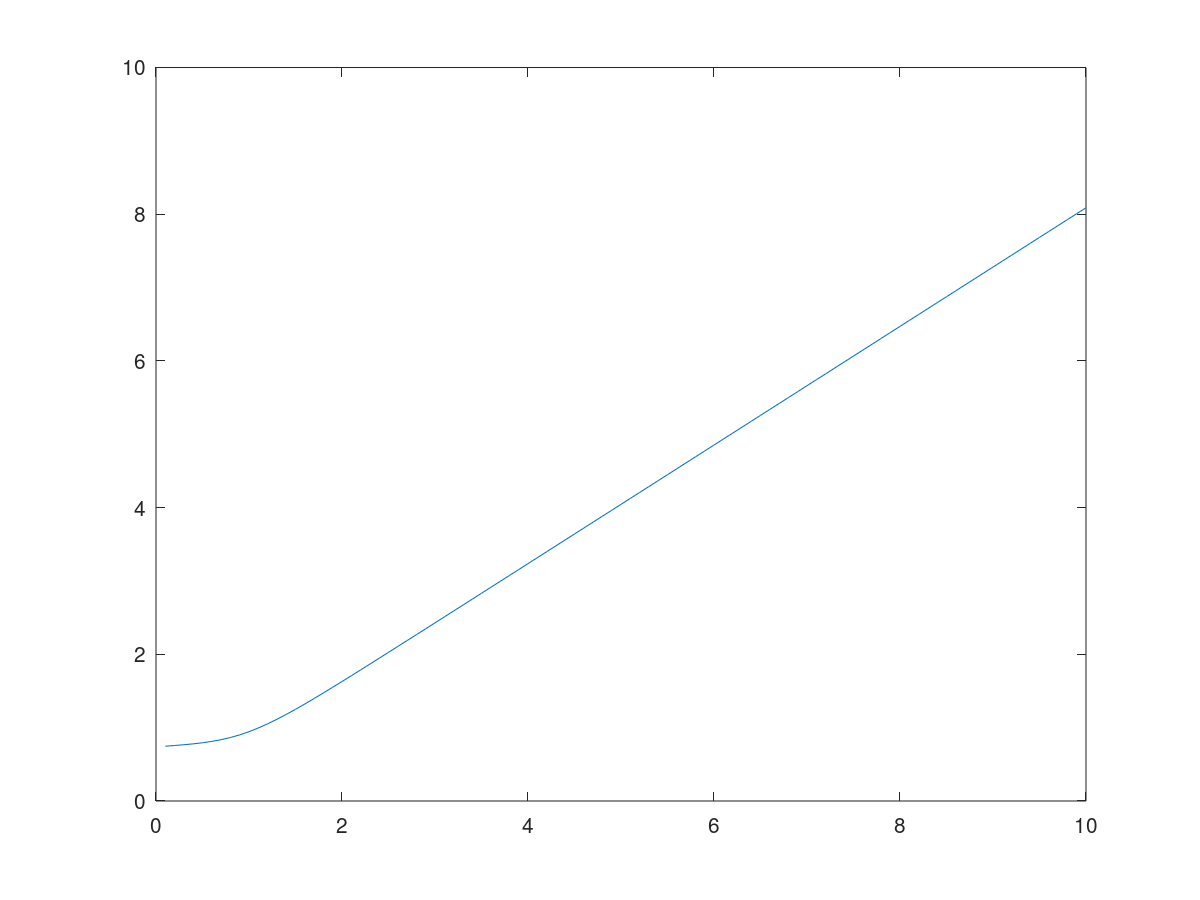
\includegraphics[scale=0.3]{plot_abh_x.png}
\label{fig:universe}
\caption{Dominanter Eigenwert abhängig von x}
\end{figure}

\subsubsection{}
Bei einem Wert von ungefähr 1.2 ist der dominante Eigenwert grösser als 1 und somit sinnvoll.

\subsubsection{}
\begin{lstlisting}
min = 0.9;
cur = 1;
max = 1.2;
format long;

i = 0;
while i < 10000
  i += 1;
  M = x_abhangig_schild(cur);
  fin = eig_dom(M)(1,1);
  diff = fin - 1;
  if abs(diff) <= 10^-15
    break
  elseif diff > 0
    max = cur;
    cur = (max + min)/2;
  else
    min = cur;
    cur = (max + min)/2;
  endif
endwhile

cur
\end{lstlisting}

Output: 1.108695552170977

\subsection{Schutz für die Unechte Karettschildkröte 2}

\subsubsection{}
\[
Jahr 1
  \begin{pmatrix}
    0 \\
    100 * u_1 \\
    0 \\
    0 \\
    0 \\
    0 \\
  \end{pmatrix}
Jahr 2
  \begin{pmatrix}
    0 \\
    100 * u_1 * u_2 \\
    0 \\
    0 \\
    0 \\
    0 \\
  \end{pmatrix}
Jahr 8
  \begin{pmatrix}
    0 \\
    100 * u_1 * u_2^7 \\
    0 \\
    0 \\
    0 \\
    0 \\
  \end{pmatrix}
\]

\subsubsection{}
\[
Jahr 1
  \begin{pmatrix}
    100 \\
    100 * u_1 \\
    0 \\
    0 \\
    0 \\
    0 \\
  \end{pmatrix}
Jahr 2
  \begin{pmatrix}
    100 \\
    100 * u_1 + 100 * u_1 * u_2\\
    0 \\
    0 \\
    0 \\
    0 \\
  \end{pmatrix}
Jahr 8
  \begin{pmatrix}
    100 \\
    100 * (u_1 + \sum_{k=1}^{6} u_2^k * u_1) \\
    100 * u_2^7 * u_1 \\
    0 \\
    0 \\
    0 \\
  \end{pmatrix}
\]

\subsubsection{}
\Large {
$$\frac{u_2^7 * u_1}{u_1 + \sum_{k=1}^{6} u_2^k * u_1} 
= \frac{u_2^7}{1 + \sum_{k=1}^{6} u_2^k}$$ \\
$$= \frac{u_2^7}{1 + \frac{1 - u_2^7}{1 - u_2}-1} =
 \frac{u_2^7 - u_2^8}{1-u_2^7} = 0.040459$$
}

\subsubsection{}
\Large {
$$\frac{u_k^{d_k} - u_k^{(d_k+1)}}{1-u_k^{d_k}}$$
}

\subsubsection{}
(u**d-u**(d+1))/(1-u**d)
\[
    \begin{pmatrix}
     0.67470 \\
     0.048593 \\
     0.014884  \\
     0.051833 \\
     0.89010 \\
     0.89010 \\
     0.00033237 \\
    \end{pmatrix}
\]

\subsubsection{}
\normalsize
\begin{lstlisting}
function retval = NextStep (u, d)
  retval = u**d / ((1-u**d)/(1-u));
endfunction


function L = L_estimate (d, u, g)
  L = zeros(length(d));
  
  #Alle die weiter gehen einsetzen
  for i = 1:length(d)-1
    L(i+1, i) = NextStep(u(i), d(i));
  endfor
  
  #Alle die in derselben Gruppe bleiben einsetzen
  for i = 1:length(d)-1
    L(i,i) = (1 - (L(i+1,i) / u(i)) ) * u(i);
  endfor
  
  #Neugeborene
  for i = 1:length(d)
    L(1,i) = g(i);
  endfor
  
  #Letzte Gruppe (Ausnahmefall)
  L(length(d),length(d)) = u(length(d));
endfunction
\end{lstlisting}

\subsubsection{}
\Large
\[
    \begin{pmatrix}
     u_1 \\
     u_2 \\
     u_3 + p  \\
     u_4 + p \\
     u_5 + p \\
     u_6 + p \\
     u_7 + p \\
    \end{pmatrix}
\]

\normalsize

\subsubsection{}
\begin{lstlisting}
x = [];
elements = 100;

p = 0;
d = [1; 7; 8; 6; 1; 1; 30];
u = [0.6747; 0.7857; 0.6758; 0.7425; 0.8091; 0.8091; 0.8091];
g = [0; 0; 0; 0; 127; 4; 80];


for i = 1:elements
  p = linspace(0,0.5,elements)(i);
  x(i) = eig_dom(L_estimate_TED(p, d, u, g))(1);
endfor
plot(linspace(0,0.5,elements), x);
\end{lstlisting}

\begin{figure}[H]
\centering
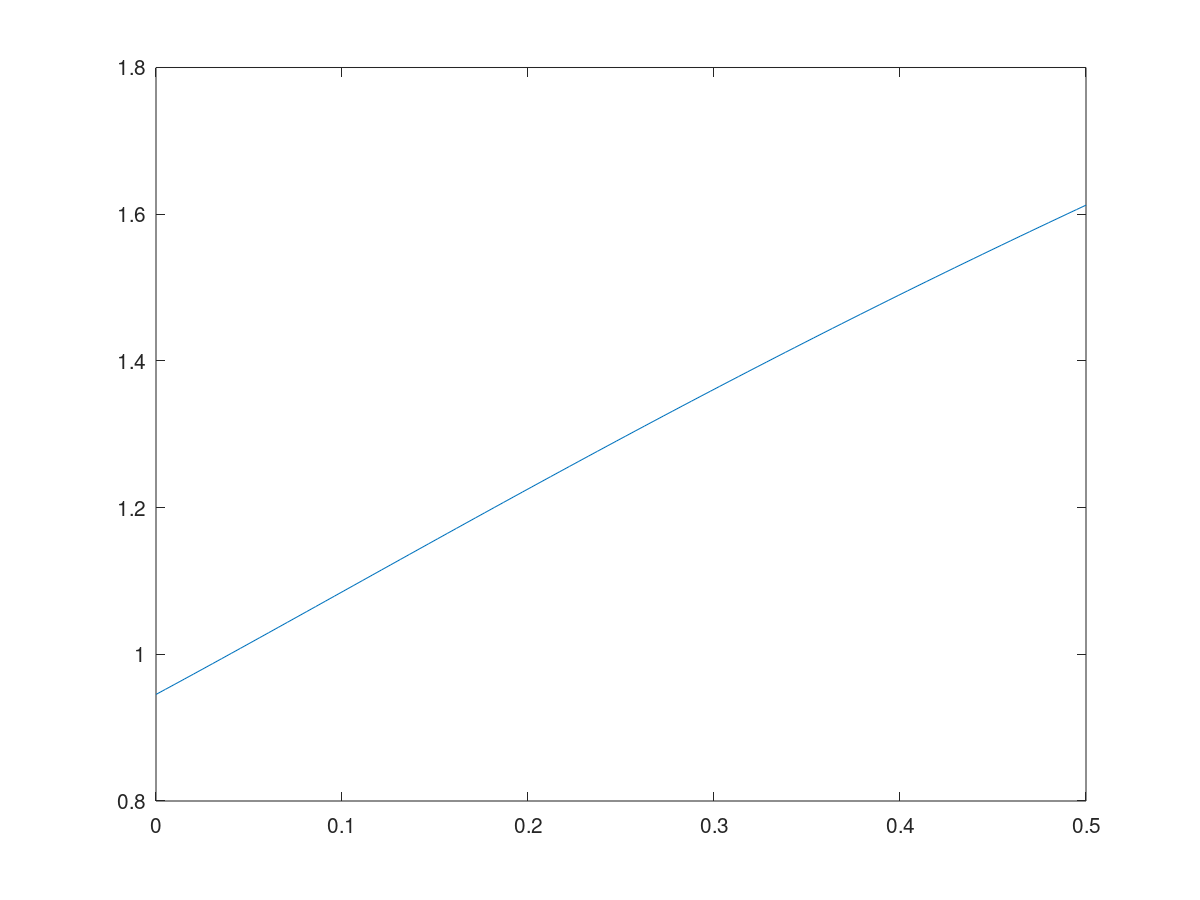
\includegraphics[scale=0.3]{dom_eig_abh_p_KARETT.png}
\label{fig:universe}
\caption{Dominanter Eigenwert abhängig von p}
\end{figure}

\subsubsection{}
\begin{lstlisting}
p = 0;
d = [1; 7; 8; 6; 1; 1; 30];
u = [0.6747; 0.7857; 0.6758; 0.7425; 0.8091; 0.8091; 0.8091];
g = [0; 0; 0; 0; 127; 4; 80];

p_min = 0;
p_max = 1;
format long;
while true
  p = (p_min + p_max)*0.5;
  currentValue = eig_dom(L_estimate_TED(p, d, u, g))(1);
  if abs(currentValue-1) <= 10^-12
    if currentValue < 1
      p_min = p;
      p = (p_min + p_max)*0.5;
    endif
    break;
  elseif currentValue > 1
    p_max = p;
  else
    p_min = p;
  endif
endwhile
p
eig_dom(L_estimate_TED(p, d, u, g))(1)
\end{lstlisting}
Output:
    p = 0.03955436545402335
    ans = 1.000000000000753


\vspace{1cm}
\section{SARS}
\subsection{}

\subsubsection{}
Die Konstanten benennen wie viele Personen vom einem Infektionszustand zu einem anderen gelangen.
$\lambda$ Bezeichnet zum Beispiel wie viele Exposed im nächsten Schritt nicht mehr Exposed, sondern Quaratantined sind.

\subsubsection{}
$$E(t+1) = E(t) + \beta(t)(kE+I) - \lambda E(t) - \epsilon E(t) $$
$$I(t+1) = I(t) + \epsilon E(t) - \delta I(t) - \theta I(t)$$
$$J(t+1) = J(t) + \sigma Q(t) + \theta I(t) - \delta J(t) - \gamma J(t)$$
$$R(t+1) = R(t) + \gamma J(t)$$

\subsubsection{}
Keine Person wird jemals zu S zurückgehen und somit wird S(t) auf lange Sicht gesehen vernachlässigbar.

\subsubsection{}
\[
    \begin{pmatrix}
    E \\
    I \\
    Q \\
    J \\
    \end{pmatrix}
    =
    \begin{pmatrix}
     1 + k * \beta (t) - \lambda - \epsilon && \beta (t) && 0 && 0\\
     \epsilon &&  1 - \theta - \delta && 0 && 0\\
     \lambda && 0 && 1 - \sigma && 0 \\
     0 &&  \theta && \sigma && 1 - \delta - \gamma \\
    \end{pmatrix}
    * v
\]

\subsubsection{}
\begin{lstlisting}
function A = sars_mat1 (k, eps, del, lam, the, sig, gam, bet)
  A = [(1-eps-lam)+bet*k, bet, 0, 0;
        eps, 1-the-del, 0, 0;
        lam, 0, 1-sig, 0;
        0, the, sig, 1-gam-del
        ];
endfunction
\end{lstlisting}

\subsubsection{}
\begin{lstlisting}
A = sars_mat1(0.1, 2/15, 15/2100, 1/5, 1/3, 1/3, 1/21, 0.7);
[v, LAM] = eig(A);
e = eig_dom(A);
for i = 1:4
  if LAM(i,i) == e
    eig_v = v(:,i);
  endif
endfor
verhalten = eig_v/sum(eig_v)
\end{lstlisting}
Output:
    e = 1.0060
    
    verhalten = 
    \begin{pmatrix}
        0.136688 \\
        0.052597 \\
        0.080556 \\
        0.730159 \\
    \end{pmatrix}

\subsubsection{}
\begin{lstlisting}
A = sars_mat1(0.1, 2/15, 15/2100, 1/5, 1/3, 1/3, 1/21, 0.7);

v0 = [477; 286; 191; 848];
res = [];
for i = 1:365
  res(:,i) = A^i * v0;
endfor

hold on
for i = 1:4
  plot(1:365, res(i,:))
endfor
hold off
\end{lstlisting}

\begin{figure}[H]
\centering
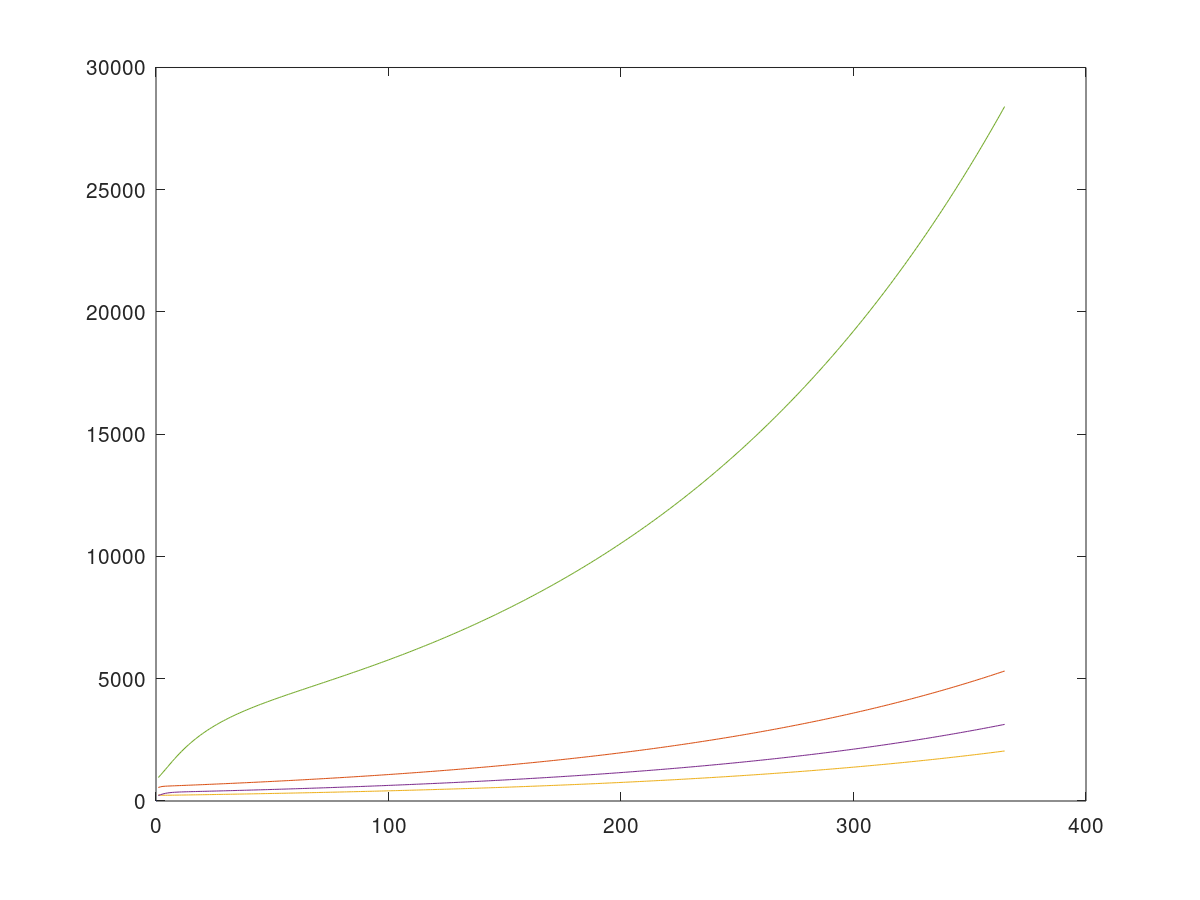
\includegraphics[scale=0.3]{SARS1g.png}
\label{fig:universe}
\caption{SARS Krankheitsverlauf (\beta = 0.7)}
\end{figure}

\subsubsection{}
\begin{lstlisting}
A = sars_mat1(0.1, 2/15, 15/2100, 1/5, 1/3, 1/3, 1/21, 0.3);

v0 = [477; 286; 191; 848];
res = [];
for i = 1:365
  res(:,i) = A^i * v0;
endfor

hold on
for i = 1:4
  plot(1:365, res(i,:))
endfor
hold off
\end{lstlisting}

\begin{figure}[H]
\centering
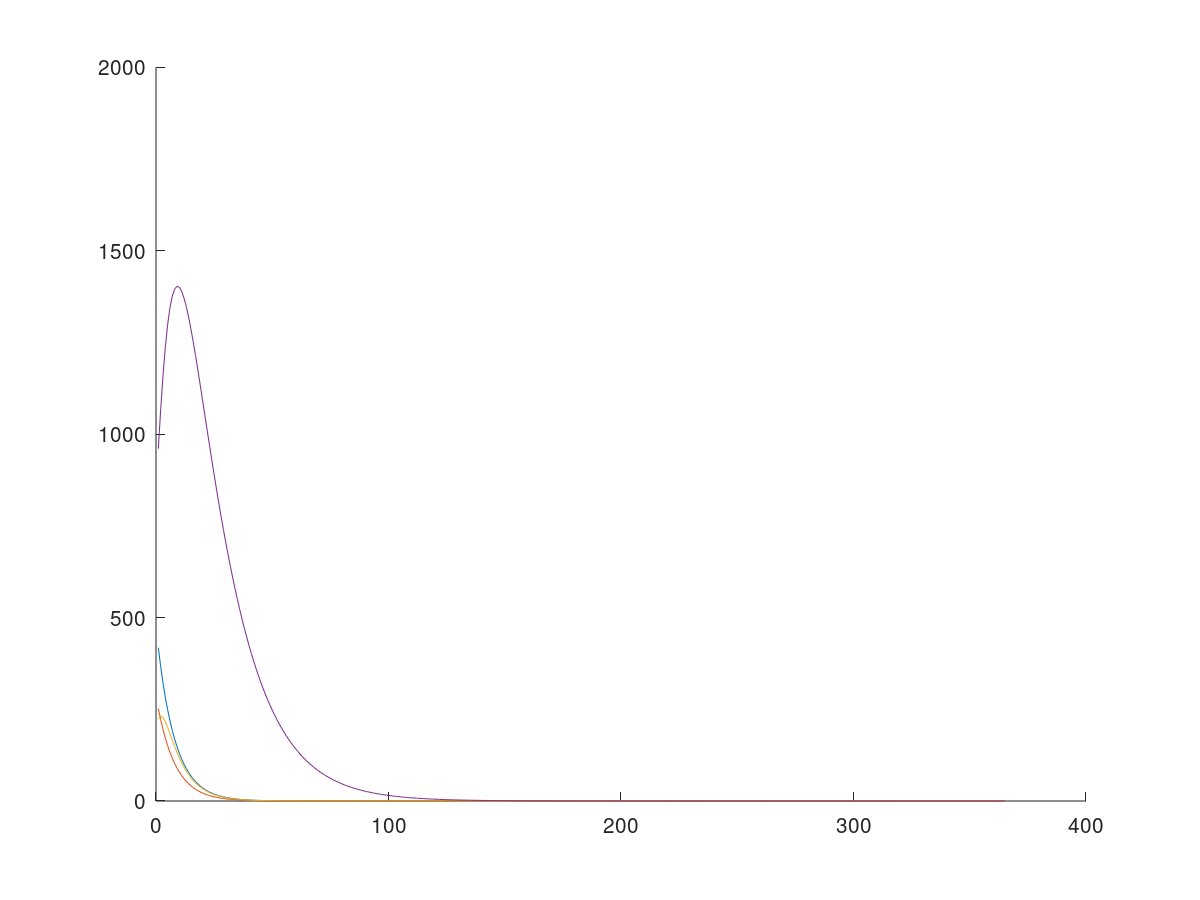
\includegraphics[scale=0.3]{SARS1h.png}
\label{fig:universe}
\caption{SARS Krankheitsverlauf (\beta = 0.3)}
\end{figure}

Man kann mit guten Hygienen, Impfungen, etc. $\beta$ niedriger machen.
Diese Methode hat einen starken Einfluss auf den Krankheitsverlauf.

\subsubsection{}
\begin{lstlisting}
bet = 0.5;
min = 0.3;
max = 0.7;
currentValue = 0;

while true
  bet = (min + max)*0.5;
  A = sars_mat1(0.1, 2/15, 15/2100, 1/5, 1/3, 1/3, 1/21, bet);
  
  currentValue = eig_dom(A)(1);
  
  if abs(currentValue-1) <= 10^-12
    if currentValue < 1
      min = bet;
      b = (min + max)*0.5;
    endif
    break;
  elseif currentValue > 1
    max = bet;
  else
    min = bet;
  endif
  
endwhile
bet
\end{lstlisting}
Output: bet = 0.6780464675219262
%TODO add graph




\end{document}
